\documentclass[]{article}
\usepackage{graphicx,array,tabu,subcaption,float,glossaries,url,amsmath}
\usepackage{geometry}
\geometry{a4paper,portrait, margin=1in}
\usepackage[T1]{fontenc}
\newcommand\numberthis{\addtocounter{equation}{1}\tag{\theequation}}
\graphicspath{{/home/shenoy/Documents/Nikhil/research/RADICAL-research/slade_paper/img/}}

\begin{document}
\title{Performance Summary of RADICAL-Pilo-YARN}
\author{Nikhil Shenoy}
\date{\today}
\maketitle

\abstract{While RADICAL-Pilot and the EnsembleMD Toolkit are self-contained software packages, their extensibility allows developers to utilize the performance benefits for other applications as well. For example, the areas of bio-molecular dynamics and genomics require capabilities for handling compute-intensive and data-intensive tasks, but RADICAL-Pilot can provide only some of this functionality. These fields require a combination of the best techniques from high performance computing and from data processing platforms like Hadoop in order to achieve good results. For this reason, RADICAL-Pilot has been extended to include Hadoop and the associated YARN resource management system to take advantage of RADICAL-Pilot's high performance computing applications and Hadoop's data management capabilities. In this paper, we compare the performance of RADICAL-Pilot with RADICAL-Pilot extended with YARN to demonstrate the usefulness of the additional functionality.}

\section{Introduction}
	RADICAL-Pilot is a Python API developed by the RADICAL-Cybertools group that aids developers in submitting and running batches of tasks on high performance machines. The API achieves this through a container called a Pilot; this container is assigned the information associated with each task in the batch, such as the location of input data and what simulation to run, and is then placed in the queue of an HPC machine. Once the scheduler on the HPC machine schedules the Pilot onto a resource, the Pilot will then start its own Agent to begin carrying out the batch of tasks. It aggregates all the necessary resources, and then pulls additional information about each task from MongoDB. The Agent is responsible for carrying out the execution for each task and making sure that the output is sent back to the user.

	\begin{figure}[H]
		\centering
		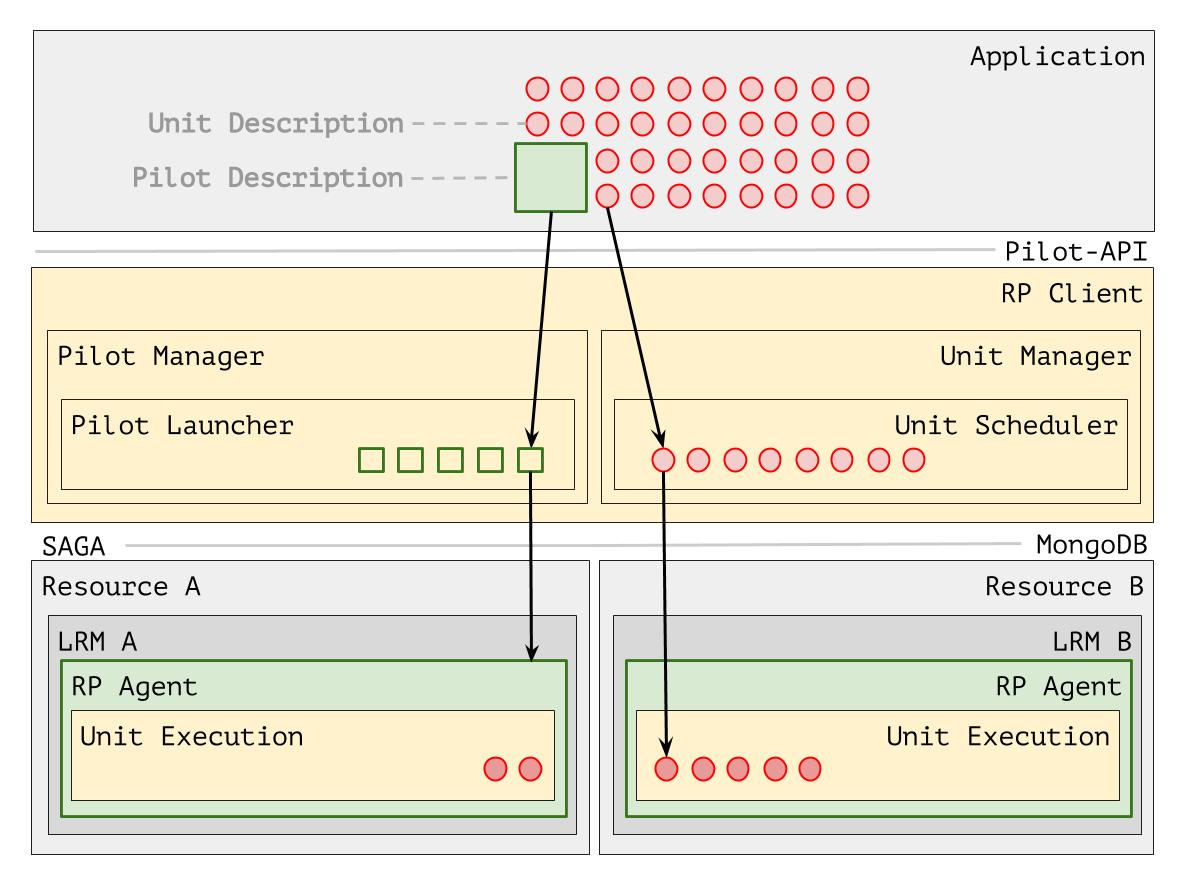
\includegraphics[width=7cm,height=5cm]{rp_arch}
		\caption{The RADICAL-Pilot Architecture \cite{rp_arch}}
		\label{fig:pipeline_block_diagram}
	\end{figure}

	This method of scheduling tasks provides many advantages, one of which is circumventing the scheduler. In current submission scenarios, each task must occupy a place in the scheduling queue and must individually wait for the required resources to become available before executing. This greatly increases the total time spent in the queue for the collection of tasks, which also increases the time to completion. However, Pilots allow users to avoid this time penalty by taking advantage of late binding and sending only the Pilot through the scheduler, reducing the wait time to that of a single task. Once the Pilot is finally scheduled, the user can then employ the various execution styles provided by the API based on the nature of their application. For example, if the batch is split into two types of tasks where one must occur before the other, the API provides functionality to schedule and execute such chained tasks. This, and the other options provided by RADICAL-Pilot, presents the user with a simple but powerful interface for task execution that outstrips current methods. By permitting any executable to be associated with a task in a Pilot, the RADICAL-Pilot API is flexible enough to handle a variety of HPC tasks, making it ideal for users who regularly work on the order of thousands of simulations.

	While RADICAL-Pilot offers an improvement in efficiency for HPC tasks, it is not designed to handle data-intensive tasks. However, Apache Hadoop and YARN are able to work on problems involving large amounts of data. YARN in particular plays the roles of resource manager and scheduler in this context, and contributes the main functionality for wrestling with large volumes of data \cite{apache_hadoop_yarn}. RADICAL-Pilot has been extended with YARN in order present an iterface which has performs well on HPC and data-intensive tasks. The extension has been implemented at the level of RADICAK-Pilot's Agent, the entity responsible for coordinating execution on the remote machine, within several components. The Local Resource Manager now retrieves new environment variables that detail the number of cores to be used on each node and the assignment of nodes, among other parameters. It then passes this information on to the newly started Hadoop and YARN demons, which examine and record the current state of the cluster.

	\begin{figure}[H]
		\centering
		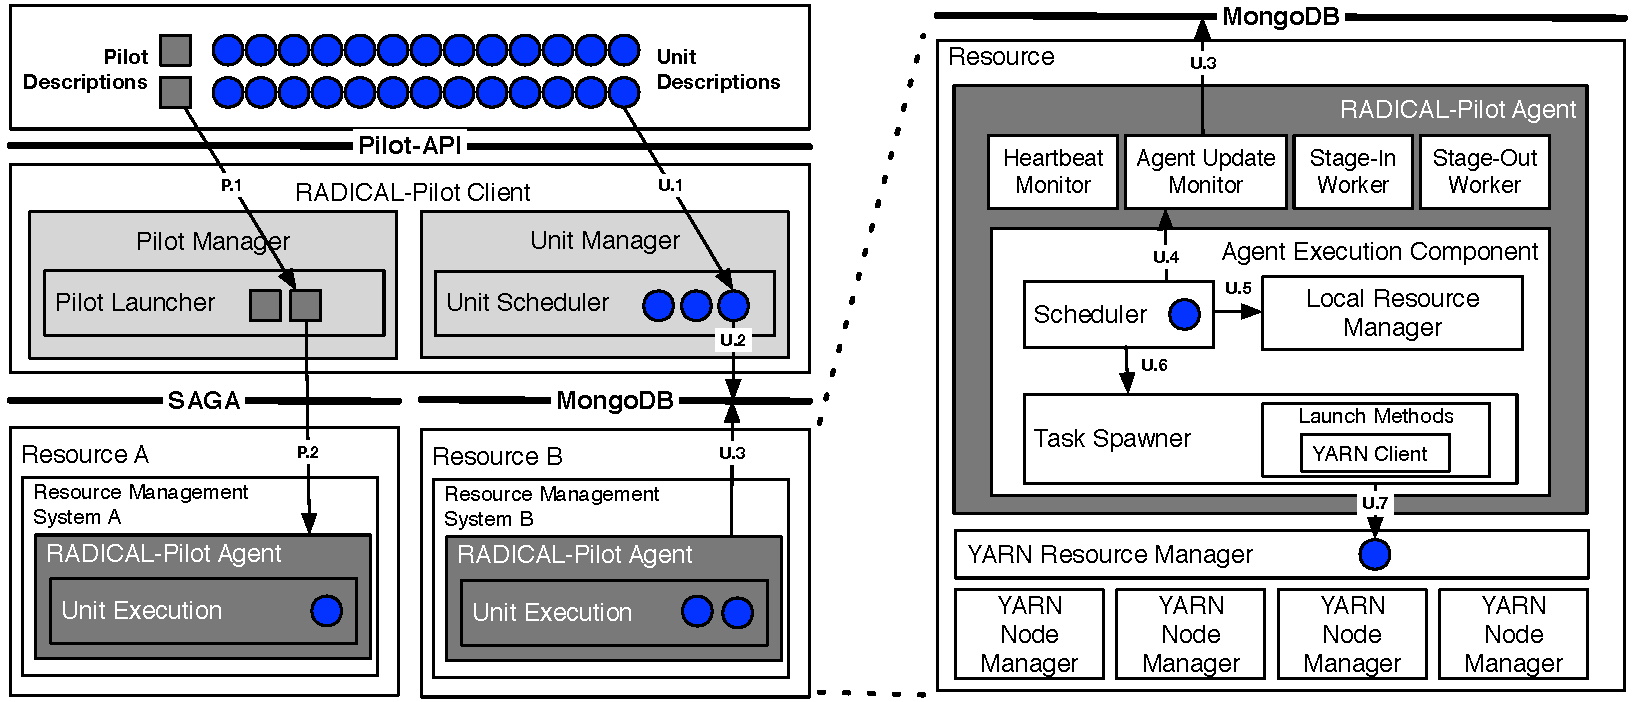
\includegraphics[scale=.42]{rp-architecture-yarn.pdf}
		\caption{The RADICAL-Pilot-YARN Architecture. As seen in \cite{hadoop_paper}.}
		\label{fig:rp_yarn_arch}
	\end{figure}

	The RADICAL-Pilot scheduler has also been updated to include information about the current state of the cluster, including updates on the total memory available and the total number of cores in use. The scheduler then uses this state information to schedule the next task appropriately. Finally, the Application Manager, which handles the resource allocations, works with the YARN Resource Manager in order to coordinate the execution of tasks. RADICAL-Pilot provisions a Compute Unit with a Description that contains the resource requirements, and then requests that YARN create a container for it. By placing the Compute Unit within the YARN container, the YARN scheduler can then easily assign the container the optimal resources for execution \cite{hadoop_paper}. 

	\begin{figure}[H]
		\centering
		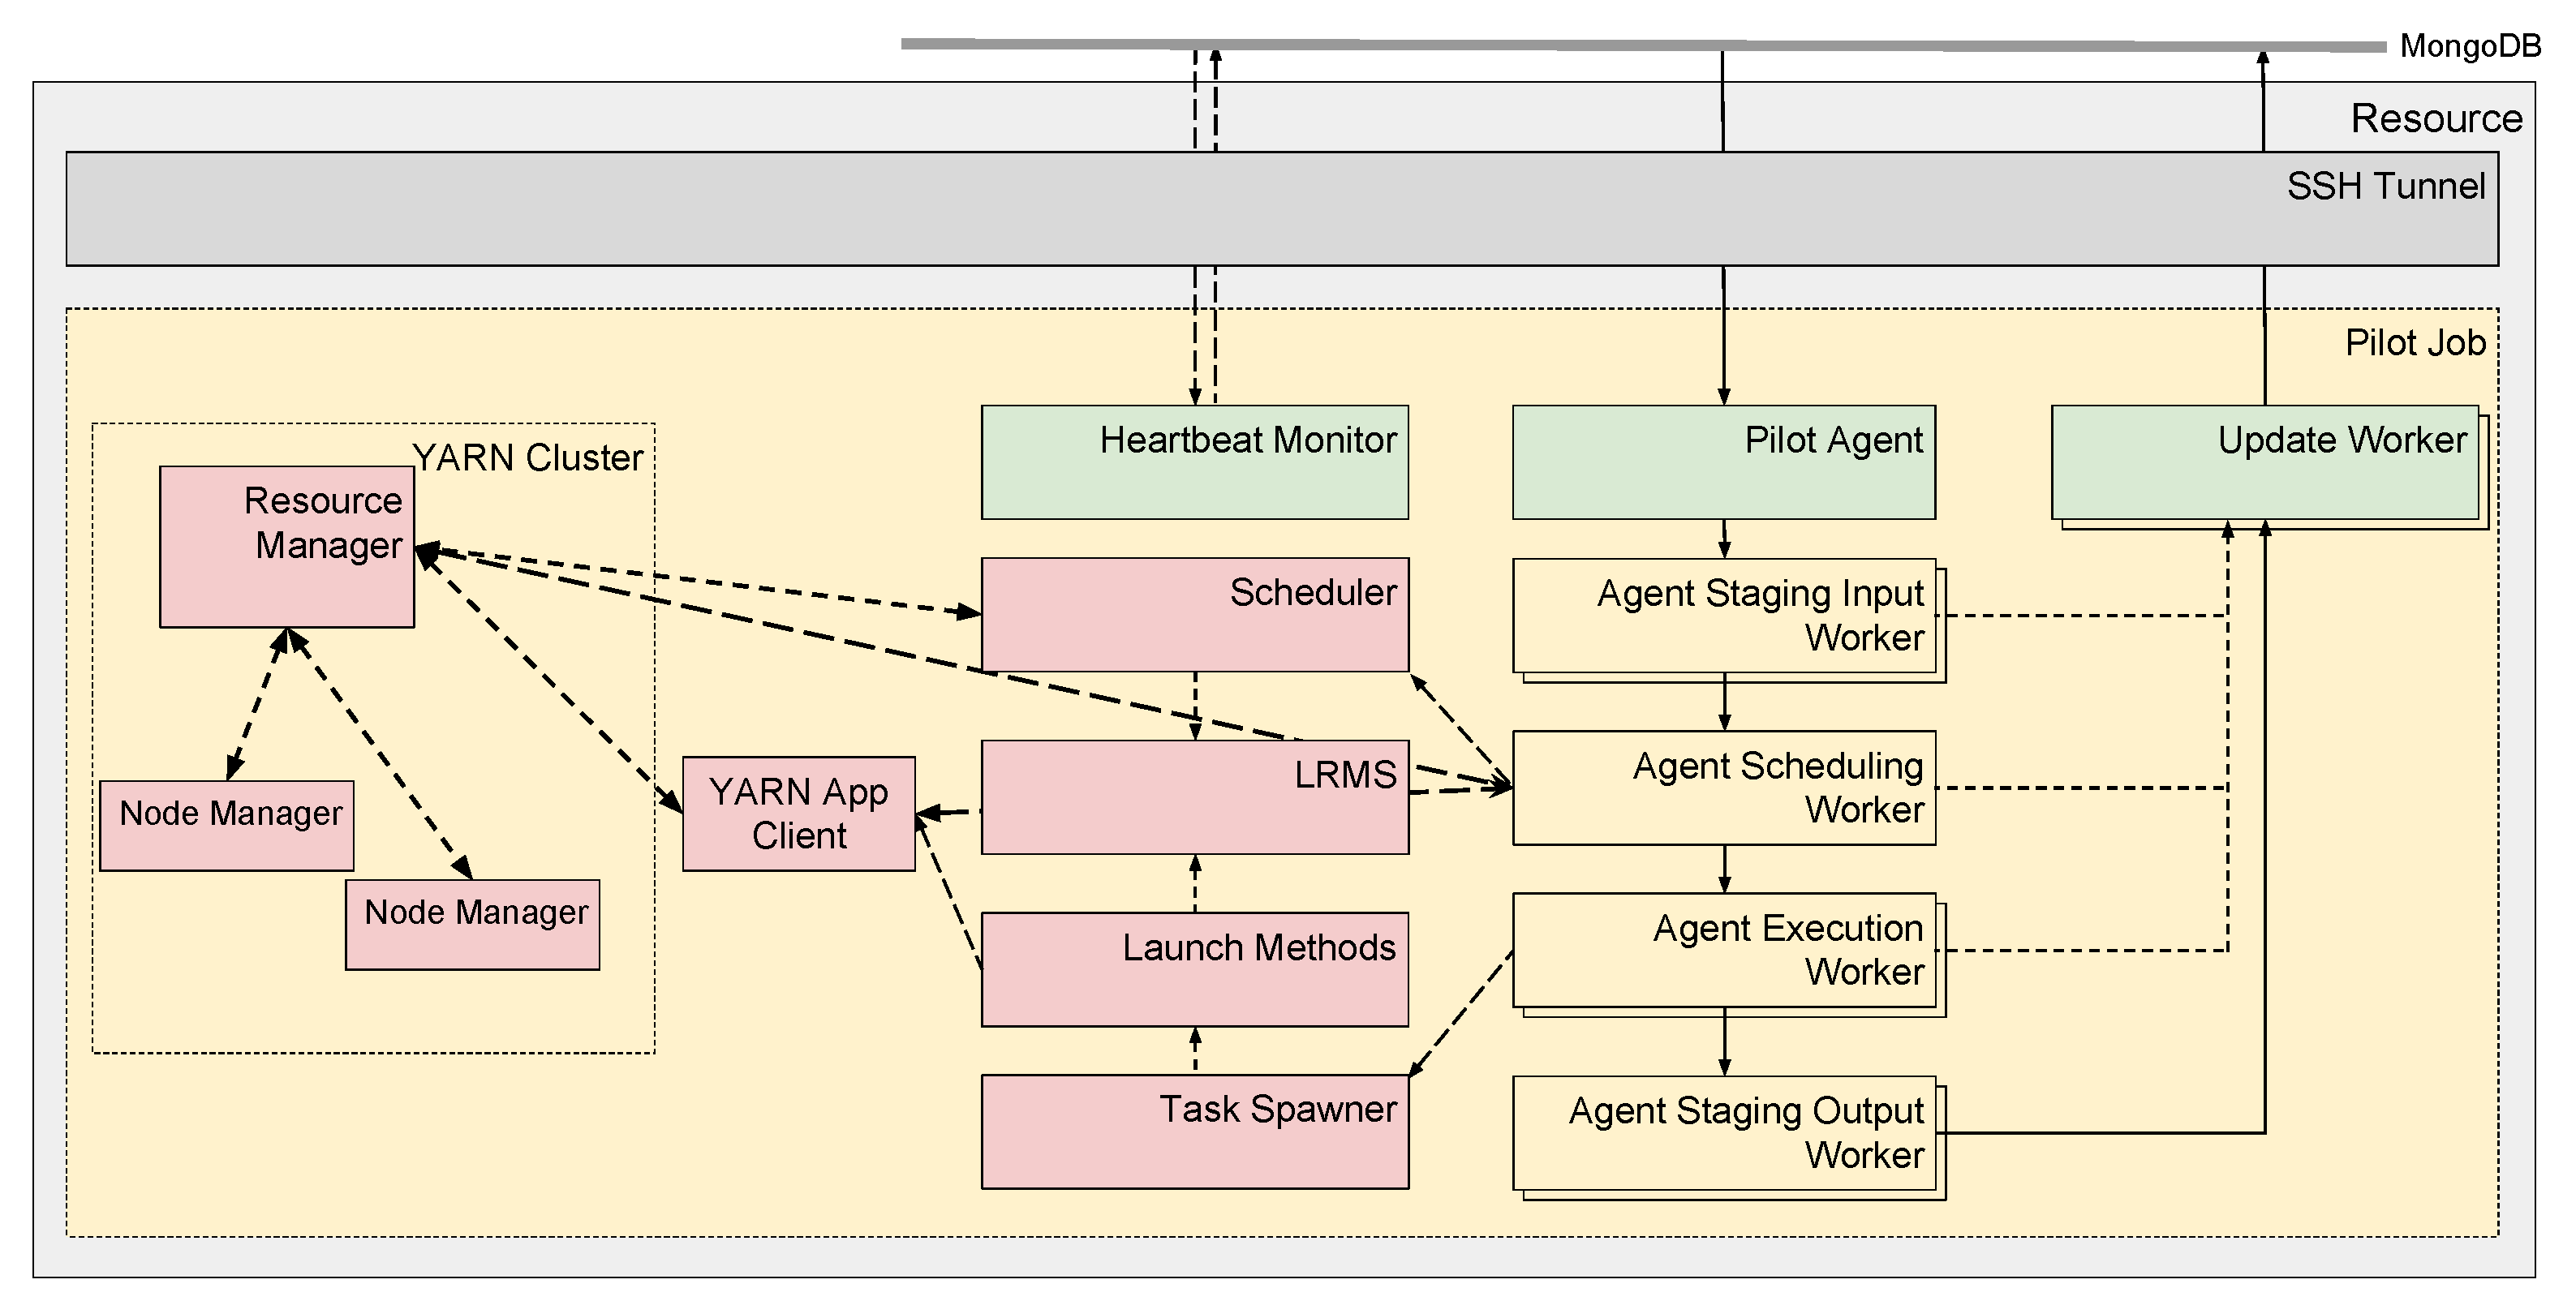
\includegraphics[scale=.22]{RP_YARN_Interaction_Diagram.pdf}
		\caption{The interaction between RADICAL-Pilot and YARN. As seen in \cite{hadoop_paper}.}
		\label{fig:rp_yarn_interaction}
	\end{figure}

	These extensions to RADICAL-Pilot give birth to they RADICAL-Pilot-YARN package, which contains functionality to operate on HPC and data-intensive tasks. In this paper, we will examine the performance of RADICAL-Pilot-YARN in comparison to RADICAL-Pilot by itself. We will do this through a simulation with a simple clustering algorithm.

\section{Experiments}

	Our experiments to compare the two softwares involve running the K-means algorithm using a varying number of clusters and points in order to judge performance capabilities. We first summarize the algorithm, and then detail the experiment configuration in Table \ref{table:config_table}.

	\subsection{Algorithm and Configuration}
		The K-means algorithm seeks to iteratively classify a set of data points in to k different clusters. It starts by placing k centroids as far away from each other as possible, but still making a first approximation of the possible classifications. Then every data point is assigned to the nearest centroid based on distance. Once this is done, a new set of k centroids is determined based on the previous assignments \cite{k_means}. Over many iterations, the centroids will eventually converge to their proper locations. The iteration is done by minimizing an error function:

		\[ J = \sum_{j=1}^{k} \sum_{i=1}^{n} \lVert \textbf{x}_{i}^{(j)} - \textbf{c}_j \rVert ^ 2\]

		where $\lVert \textbf{x}_{i}^{(j)} - \textbf{c}_j \rVert ^ 2$ represents the distance between centroid $\textbf{c}_j$ and the data point $\textbf{x}_{i}^{(j)}$. The result are k different points that represent the optimal classifications fo the data set.

		\begin{table}[H]
			\centering
			\begin{tabu}{|c|c|}
				\hline
				Parameter & Value \\ 
				\hline
				\hline
				RADICAL-Pilot Version & v0.40.1-41-g6101f4a \\
				\hline
				Target Machine & XSEDE Stampede \\ 
				\hline
				Iterations of K-Means & 2\\ 
				\hline
				Cores & [8,16,32]\\
				\hline
				Tasks & [8,16,32]\\
				\hline
				Clusters & [50,500,5000] \\
				\hline
				Total Data Points & [10000,100000,1000000]\\
				\hline
				Data sets & \url{dataset_100K_3d.in}, \url{dataset_10K_3d.in}, \url{dataset_1M_3d.in}\\
				\hline
			\end{tabu}
			\caption{Experiment Parameters}
			\label{table:config_table}
		\end{table}

		% Explanation of Parameters
		Table \ref{table:config_table} shows the parameters involved in this experiment. We implement the k-Means algorithm on XSEDE's Stampede machine using RADICAL-Pilot version 0.40.1, and we run two iterations of the algorithm. We want the computational cost of the experiment to remain the same in each configuration, so we constrain the product of the number of clusters and the number of data points to be constant. Doing this, we run the algorithm on configurations of 50 clusters and 1,000,000 points, 500 clusters and 100,000 points, and 5000 clusters and 10,000 points. Each of these points is represented by a vector of length three, which is commonly used to describe the locations and velocities of particles in three dimensional space. We run each configuration using 8, 16, and 32 cores each, and we set the number of tasks equal to the number of cores. Finally, we run this entire configuration using both RADICAL-Pilot and RADICAL-Pilot-YARN. This set up of the experiment allows us to examine the scaling behavior of both softwares in terms of the number of cores, and to compare the performance of each under identical conditions.

		% Pilot-State Mapping
		In this experiment, we only track the time-to-completion for each software. Measuring individual components is not necessary here, as the experiment is intended to present the two softwares as black boxes and requires the user to pay attention only to how fast his script is completed. However, one can see what states the time-to-completion measurement encompasses in Figure \ref{fig:pilot_state_mapping}.

		\begin{figure}[H]
			\centering
			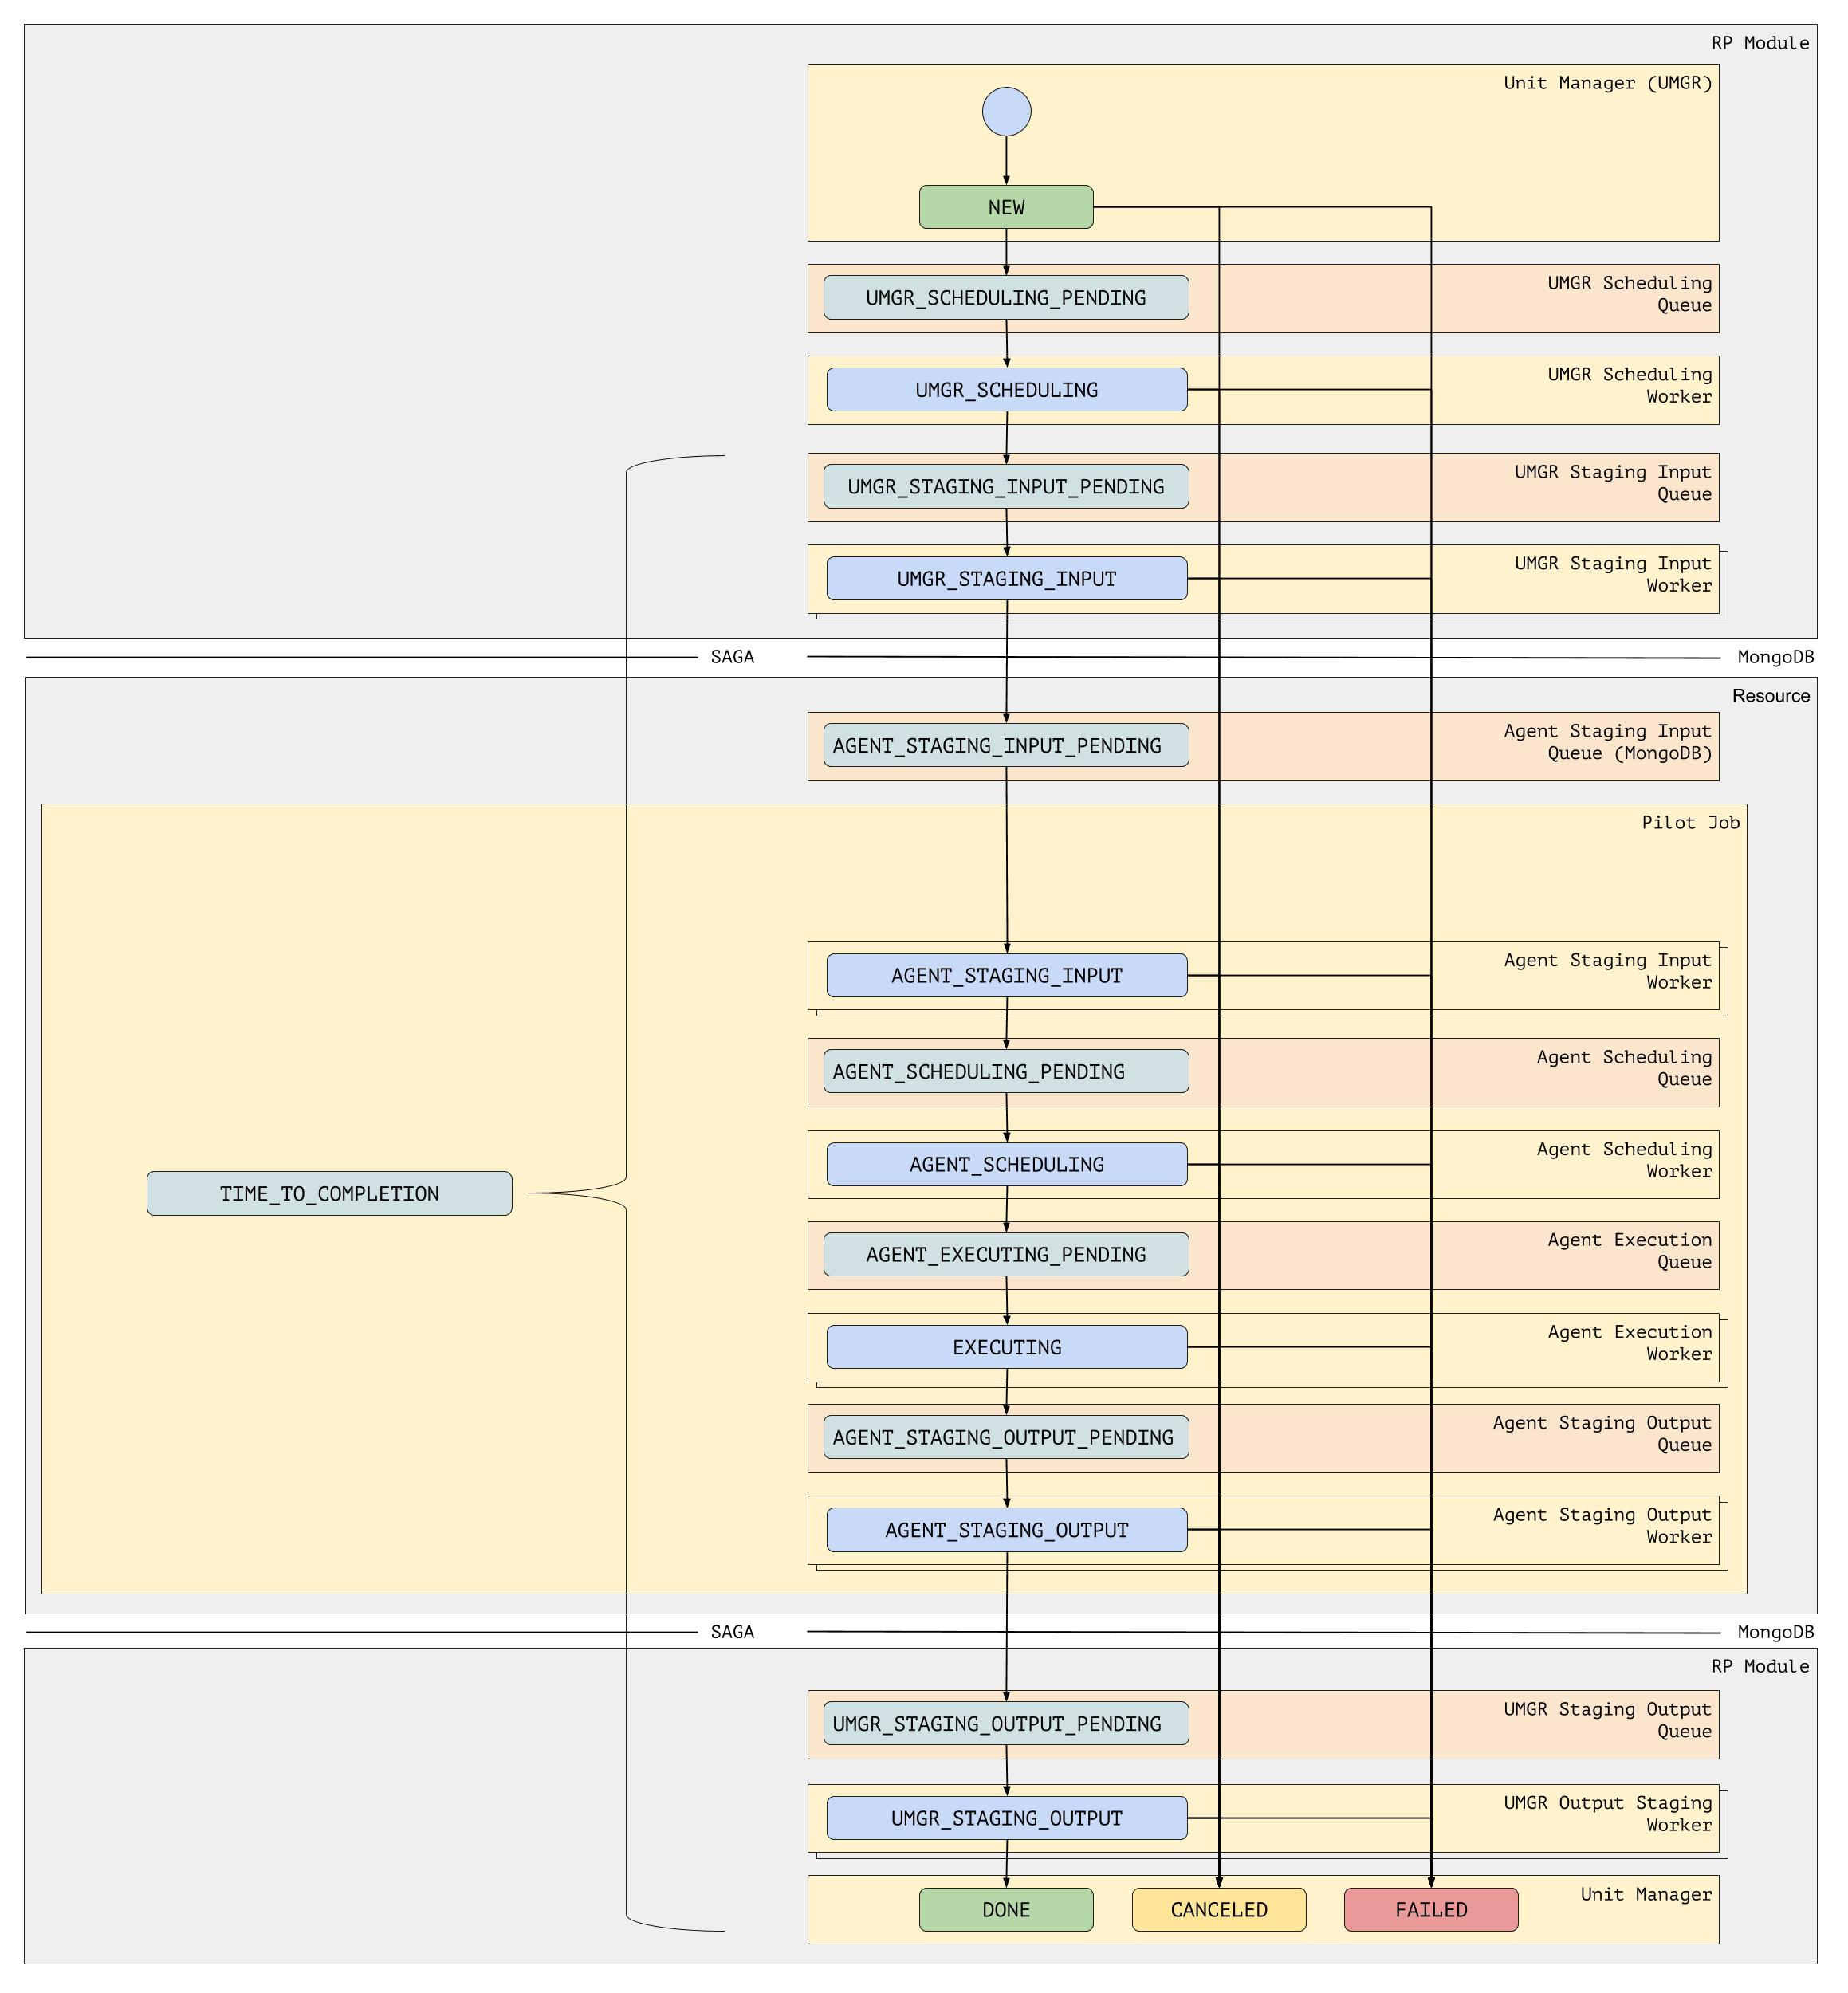
\includegraphics[scale=.19]{rp_state_model_mapping.jpg}
			\caption{Mapping of parameters to pilot state model. Derived from \cite{rp_state_diagram}.}
			\label{fig:pilot_state_mapping}
		\end{figure}

		As shown in Figure 2, the time-to-completion encompasses almost all of the states that the Pilot transitions through. This includes the staging of input for the Unit Manager and Agent, scheduling and executing simulations, and then staging the resultant data out to the Agent and Unit Manager. Formally, we state the time-to-completion in Equation 1:

		% Measurement equation
		\begin{align*}
			Time\_to\_Completion = DONE - UMGR\_STAGING\_INPUT\_PENDING \numberthis \label{1}
		\end{align*}

		This measurement, taken in seconds, provides us with the time necessary to complete a user's tasks.

	% Graphs and Analysis
	\subsection{Analysis}

		For each configuration of points and clusters, we graphed the time-to-completion across all cores.

		\begin{figure}[H]
			\centering
			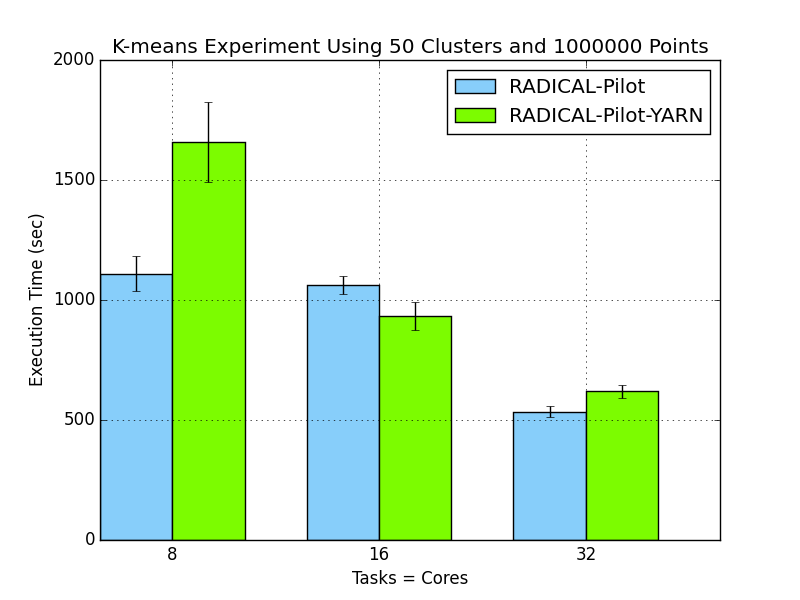
\includegraphics[scale=.50]{50.png}
			\caption{50 clusters, 1,000,000 points}
			\label{fig:50}
		\end{figure}

		In the configuration with 50 clusters, the first trend that we noticed is that the time-to-completion decreases as the core count increases. This is expected, since holding the total amount of computation the same and increasing the core count classifies this experiment as an instance of strong scaling. We observe this for both softwares. However, the comparisons between RADICAL-Pilot and RADICAL-Pilot-YARN do not yield a consistent pattern of increased performance in favor of RADICAL-Pilot-YARN. In the case with 8 cores, the time-to-completion for RADICAL-Pilot-YARN far outstrips that of RADICAL-Pilot, which is counter to the design goals RP-YARN. Scaling up to 16 cores, we notice that the relationship between the two softwares is reversed. RP time-to-completion exceeds that of RP-YARN in a range of about 20-200 seconds, within error bars. The comparison is decidedly in favor of RP-YARN, since it's time-to-completion is lower. In the case with 32 cores, the relationship reverts back to being in favor of RP. Yet, contrast in the execution times is much less than it was in the first case, indicating a difference of at most 200 seconds.

		\begin{figure}[H]
			\centering
			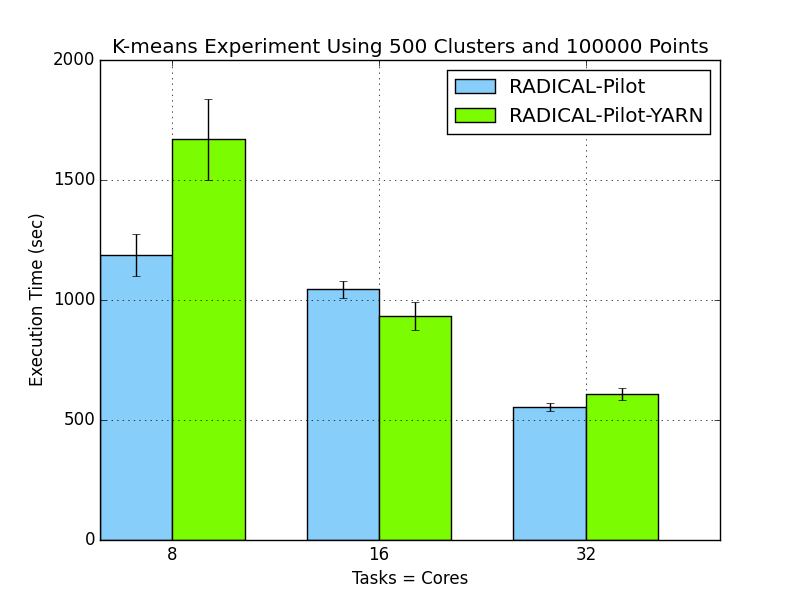
\includegraphics[scale=.50]{500.png}
			\caption{500 clusters, 100,000 points}
			\label{fig:500}
		\end{figure}

		Figure \ref{fig:500} shows the scaling behavior for the 500 cluster, 100,000 point case. The plots for the 500 and 50 cluster cases are remarkably similar. The 8 core case showed an increase in execution time for both RP and RP-YARN in comparison to the 50 cluster, 8 core case, but otherwise showed a similar disparity of time between the two softwares. RP execution time decreased slightly between the configurations for the 16 core case, but error bars indicate that RP statistically still takes longer than RP-YARN to run. Finally, the 32 core case shows a decrease in execution time for RP but an increase for RP-YARN, accentuating the relationship observed in the 50 cluster configuration. In summary, while there were fluctations in the times-to-completion of each execution, this configuration of cluster and points reinforced the trends noticed in the 50 cluster case. 

		\begin{figure}[H]
			\centering
			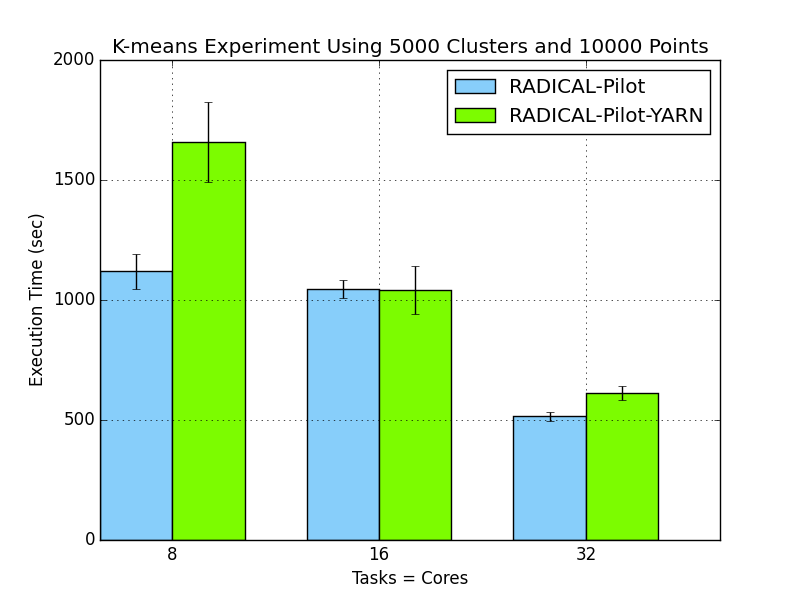
\includegraphics[scale=.50]{5000.png}
			\caption{5000 clusters, 10,000 points}
			\label{fig:5000}
		\end{figure}

		The 5000 cluster case also showed similarities to the trends in the 50 cluster and 500 cluster cases, as shown in Figure \ref{fig:5000}. Again, we see a large disparity in the execution times of RP and RP-YARN at 8 cores, ranging from 300 seconds to 700 seconds. The ratio between the two times relatively constant when compared to the 50 and 500 cluster cases. At 16 cores, we notice that the times-to-completion are almost identical, but the error bars give us more insight into the behavior. Since the error bar for RP-YARN is larger than that of RP, it is possible that the time-to-completion for RP-YARN may fluctuate between being greater than, less than, and equal to the time-to-completion for RP. At 32 cores, we see the largest difference of the three configurations between RP-YARN and RP, with a range of at most 200 seconds. Again, this supports the trends found in the other two cases. 


		Holding the number of cores at 8 and comparing across the number of clusters, we see almost no change in the execution time for RADICAL-Pilot-YARN. This is expected, since the total amount of computation is constant across all configurations of points and clusters. In comparison, the RADICAL-Pilot execution time fluctuates more. However, the disparity between the two softwares is significant between all configurations, indicating the likelihood that RADICAL-Pilot-YARN actually outperforms RADICAL-Pilot for this configuration of k-Means and cores. We see similar results when comparing the different configurations in the 16 core case. The difference between RADICAL-Pilot and RADICAL-Pilot-YARN is not as pronounced, resulting in execution time ratios that approach unity. In the 5000 cluster case, the time for both RP and P-YARN are essentially identical, but the error bars of RP-YARN enclose those of RP, rendering this measurement as suspect. Finally, the 32 core cases show again that the RP-YARN execution times stay almost exactly constant while the RP times waver in final value.

		The slight fluctuation of the results RP can be attributed to a variety of reasons, with one being a difference in the version of RP being used. The original experiments in \cite{hadoop_paper} were performed six months before the writing of this paper, so the observed speedups could be attributed to updates in the implementation of RADICAL-Pilot. While the RADICAL-Pilot version may have changed, the RADICAL-Pilot-YARN version and configuration most likely has been unchanged, which would explain why all the YARN results are nearly identical to those obtained in the Hadoop on HPC paper. Another possibility might be a lack of iterations. Perhaps running each configuration of clusters, points, and cores at least five times and observing the execution times generated by each run would paint a more accurate picture of the behavior of RADICAL-Pilot. It is possible that the values recorded here are statistical outliers and not representative of the true behavior of the software. To verify this, additional testing iterations will be performed. 

	% Reproducibility
	\subsection{Reproducibility}
		The experiments we performed can be replicated using the code located at \url{https://github.com/Nikhil-Shenoy/RADICAL-research/tree/master/yarn_replication/output_data}.

		The exact steps are as follows:
		\begin{enumerate}
			\item Set up virtual environment on local machine using \url{virtualenv} tool.
			\item Install RADICAL-Pilot using the instructions found in the documentation at: \\
				  \url{https://radicalpilot.readthedocs.io/en/stable/installation.html}
			\item Acquire an account on the remote target machine. In this case, the target machine was XSEDE's Stampede.
			\item Generate a free MongoDB instance using MongoLab (\url{https://mlab.com/}) and note its access URL.	
			\item No modifications to any of the Python files is required, unless there are problems with loading modules. If this is the case, then one should modify the instructions in the \url{pre_exec} phase of the Compute Unit to clear all modules and then reload the required modules.
			\item Once all modifications are made, the application can be started by passing the appropriate arguments to the \url{k-means.py} script. The parameters (in this order) are:
				\begin{itemize}
					\item Number of clusters
					\item Number of elements in each vector data point
					\item Number of cores to be used
					\item Number of tasks to be run
					\item Input data file
					\item Name of the output profile
					\item Name of scheduling queue
					\item Name of remote machine
				\end{itemize}
			\item To run all the configurations test for this paper, simply run the \url{run_yarn.py} script. This file cycles through and runs all of the 18 configurations displayed in the plots without requiring any additional parameters.
			\item Use Tmux or another terminal multiplexer to start the job from your machine. You can detach the job once it begins executing on the remote target machine. It is recommended to start the job at night, as it will be completed by the next morning.
			\item If any errors occur while testing, remember to safely close and stop the RADICAL-Pilot script. Also make sure that the requrested resources are not still associated with one's account on the remote machine. One can verify this by logging in to that machine and checking the job status.
			\item Remember to run all jobs with the following environment variables:
				\begin{itemize}
					\item RADICAL\_PILOT\_VERBOSE=DEBUG
					\item RADICAL\_PILOT\_DBURL= <your mongodb url>
				\end{itemize}
		\end{enumerate}

\section{Conclusion}

	This set of experiments was conducted to attempt to verify the performance benefits of the YARN extension to RADICAL-Pilot over the RADICAL-Pilot module by itself. We measured the time-to-completion of the different configurations of k-Means clustering as a way to simulate a user's experience with both softwares and tried to empirically demonstrate the capabilities of the new extensions. While the theory and design decisions behind RADICAL-Pilot-YARN are sound, the evidence that we found through our experiments currently does not support it. On the other hand, the data does not decisively reject the expectation that RADICAL-Pilot-YARN should incur a smaller time-to-completion. Across the three configurations of clusters and points, we observe that, in the cases of 8 and 32 cores, that RP-YARN always had a larger time-to-completion than that of RP by itself. However, the ratio between the execution time for RP-YARN and RP at 8 cores is larger than it is at 32 cores. This may imply that the two softwares have similar performance at high core counts, and that a difference in performance can only be noticed at lower core counts. A possible reason for this may be that an increased overhead incurred by the YARN components at lower core counts, but that penalty becomes reduced as more cores are added. The other significant trend across all configurations was that of the 16 core cases; in two out of the three, RADICAL-Pilot was observed to have a larger time-to-completion than RADICAL-Pilot-YARN. In the third case, the times-to-completion were essentially equal in mean value, but the error bars demonstrated that the RP-YARN time could fluctuate from being greater than RP to less than RP. Two immediate implications can arise out of this; if, in subsequent experiments, RP-YARN is shown to have a greater time-to-completion than RP, then the result would aid in rejecting the theory behind adding the YARN components to RADICAL-Pilot. All but two configurations of cluster, points, and cores would show that RP-YARN is outpaced by RP, suggesting that the YARN components are not necessary. Alternatively, the RP-YARN time being less than the RP time would only lead to additional inconclusive evidence, as no clear relationship between RP and RP-YARN can be established. In summary, these experiments have not been able to successfully verify the advantage of adding the YARN scheduling and resource management components to the existing RADICAL-Pilot software. The evidence seemingly indicates that RADICAL-Pilot-YARN actually slows down the performance of the system, arguing against the theoritcal underpinnings of the YARN extensions.

\section{Future Work}
	These experiments can and should be extended to analyze the full relationship between RADICAL-Pilot and RADICAL-Pilot-YARN. Verification of our experimental results would be useful to those currently developing additional YARN functionality for RADICAL-Pilot, as the performance information can suggest whether the new modules are necessary. Additional work can explore the relationship between cores and each configuration by utilizing higher core counts, machine permitting. Such an experiment would verify whether the performance of RADICAL-Pilot and RADICAL-Pilot-YARN becomes indistinguishable at larger core counts. Finally, one could perform a formal comparison between the results obtained in \cite{hadoop_paper} and our results to find out the changes made to RADICAL-Pilot in the intervening time. The additions in the six-month time period could provide insight into the behavior RADICAL-Pilot in these experiments.

\section{Lessons Learned}
	Really, the lessons I learned were not much different than those I learned from the EnsembleMD performance analysis, as the work was very similar in nature to these experiments.

	% Analyzing the performance of a system can lead to many insights about the system, and about the attitude with which one approaches experimentation in general. During our experience with testing the EnsembleMD Toolkit, we learned a variety of concepts which we believe have improved our abilities as researchers.

	% One of the most important concepts we learned about is careful design of experiments. At the beginning of our experimentation, we had a tendency to dive into the data head first without a solid plan for what we were measuring. We tried to find relationships between every pair of variables in the data set, but soon learned that this was much too inefficient to produce good results. In many of those tests, the relations we found did not yield any useful information about the system, which rendered all the time spent running those simulations useless. Not only would these types of experiments not produce results, but adding just one variable would dramatically increase the complexity of running the entire set of simulations. After this experiment, we learned to focus on specific behaviors of the system we wanted to examine, such as strong scaling, and tailored our experiments towards those. This resulted in concise, informative results that provided useful information for the development team.

	% We also understood the importance of reproducibility of experiments. Providing the parameters to reproduce an experiment allows us to go back to the experiment after some time and still expect to have the same results. Also, others can look at our work, run the same experiment, and verify whether our interpretation of the data is valid. In the greater scientific community, reproducibility allows a scientist to test the foundations on which his current experiment is based. If he thinks his experiment went wrong based on work done by others, he can go and re-run the experiment to either verify or change his assumptions. Sometimes the initial interpretation of the results was wrong, and another trial yielded a more significant, appropriate result. This allows the community to make sure that the assumptions from previous experiments are a solid foundation upon which new work can be done.

	% Adapting existing code to my experiments improved our skills as developers and widened our knowledge of EnsembleMD and the rest of the RADICAL Cybertools stack. In the all the projects we had done before joining the group, we were required to implement all functionality from scratch, which augmented my understanding of class concepts but did not reflect real software development. In designing my experiments, we were forced to look at code written by others, understand it, and adapt it to my work. As we read, we understood why layers of abstraction were implemented between components of the Toolkit, and between layers of the RADICAL Cybertools stack. Our view of the system changed from a collection of disjoint Pilot operations into a series of well-defined state transitions. Learning about the architecture in this way gave our experiments more context, and allowed us to remove measurements which didn't capture the interactions between important components. 


	% Finally, we gained a greater appreciation for reading technical papers. After we read a variety of papers written by RADICAL developers and other members of the community, we understood that impactful papers require careful design in order to be useful. In specific, the specific sections of a paper must have a clear focus and a proper transition into the following section. We especially noticed how important the introduction and background are in setting the context for the experiment. If carefully crafted, then the user will be more willing to read the rest of the paper and understand why one's work is so important. The sections describing the experiment must be detailed, yet concise. It is best to include only enough information to reproduce the experiment and explain why the work is being done; any more information could cause the reader to become confused and lose sight of the experiment's purpose. Finally, the analysis and conclusion should bridge the context laid out in the opening sections and the results from the experiment to summarize the impact of the work. While many essays and other pieces of writing do a have a similar structure, we were able to learn how the scientific community adapted that structure to fit its needs and present its work to the world. Going forward, we can make use of this in order to make our own contributions.


% Using no_cite to make sure all the bib entries are processed
% \nocite{pstar}
% \nocite{saga_paper}

\bibliography{yarn_summary}{}
\bibliographystyle{IEEEtran}		
\end{document}